\chapter{Felhasználói dokumentáció}
\label{ch:user}
\section{A téradatok verziókezelésének problémája}
Téradatokkal -vagy bármilyen kép alapú adatokkal- egyre több szakterület dolgozik, és általánosan ezek a folyamatok kifejezetten magas számú felhasználók által végzett módosítással járnak. Az információk tárolása vagy binárisan, vagy valamilyen összetett geodéziai adatbázis állománnyal történik, ezek verziókövetésére pedig nem született még igazán megoldás. A QGIS egy széles körben elterjedt, főleg térképészeti adatok létrehozását, módosítását és tárolását támogató szoftver, ami még nem rendelkezik verziókezelést megvalósító kiegészítéssel, a Q-Aegis modul ezen hiány betöltésére született.
\section{A modul működése}
A Q-Aegis plugin az AEGIS nevű téradatkezelő keretrendszer felhasználásával biztosítja a QGIS-ben létrehozott projektek műveletalapú verziókezelését. A verziókezelő és a szerkesztőprogram közti technikai különbségeket a nyílt forráskódú Python .Net modul használatával hidalja át. A program követi a rétegek és a rajtuk lévő feature-ök változásait, a geometriák alakulását reverzibilis transzformációkká alakítja és ezeket tárolja. A korábbi vagy újabb verziók betöltésekor így nem szükséges forrásfájlokat cserélni, a rétegek új állapotait beállítani, mindez automatikusan megtörténik. Ezen kívül a megvalósítása miatt a Q-Aegis plugin lehetővé teszi, hogy a QGIS-ben végzett munka során csupán az eredetileg nem menthető memóriában tárolt rétegekkel dolgozzon a felhasználó.

\section{A beépülő modul telepítése}
\subsection{Rendszerkövetelmények}
Mivel a program egy plug-in a QGIS térinformatikai programhoz, ezért használatához szükséges legalább a 3.6-os verzió jelenléte. Korábbi verziók esetén nem ismert viselkedések léphetnek fel, viszont a beépülő potenciálisan használható korábbi 3.x-es verziókkal is (nem tesztelt). Az AEGIS csomag használata miatt, amennyiben nincs még jelen a rendszerben, telepíteni kell a Microsoft .NET keretrendszert a legfrissebb verzióig. Az előbbi dependencia miatt a program csak Microsoft Windows operációs rendszer alatt használható.
\subsection{Telepítés}
A beépülő telepítése kifejezetten egyszerű, csak ki kell csomagolni a mellékelt tömörített állomány tartalmát a helyi QGIS verzió python plugin könyvtárába, amely telepítéstől függően a ../OSGeo4W64/apps/qgis/python/plugins, vagy a ../QGIS3.x/apps/qgis/python/plugins útvonalon érhető el. Ezután a QGIS-t elindítva a plugins/manage and install plugins menüponton keresztül megnyitott plugin kezelőben be kell kapcsolni a Q-Aegis plugint, hogy az ábrán látható állapotot kapjuk :
\begin{figure}[H]
	\centering
	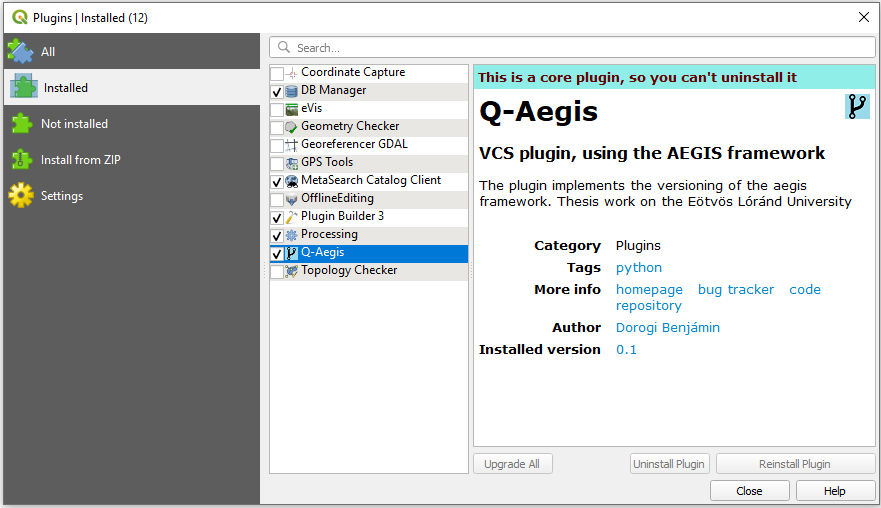
\includegraphics[width=\textwidth,height=250px]{images/enable_plugin}
	\caption{Az aktiválás utáni állapot}
	\label{fig:picture-1}
\end{figure}

Ezután a verziókezelő modul használatra kész.
	
\section{A verziókezelő használata}
\subsection{A kezelőfelület}
A beépülő modul a QGIS-en belül létrehozott projektekkel van összekötve, így amíg nem nyitunk meg egy projektet, nem érjük el az új funkciókat. Projekt megnyitása után a modul kezelőfelülete a QGIS beépülő modulok eszköztárán található ikonra (~\ref{fig:picture-2}) kattintva nyitható meg, és a (~\ref{fig:picture-3}) ábrán látható módon néz ki alapértelmezett állapotban.
\begin{figure}[H]
	\centering
	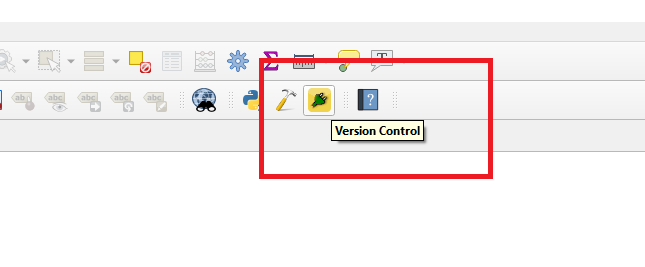
\includegraphics[width=0.8\textwidth,height=190px]{images/plugin_button.png}
	\caption{Az eszköztáron található ikon}
	\label{fig:picture-2}
\end{figure}
\begin{figure}[H]
	\centering
	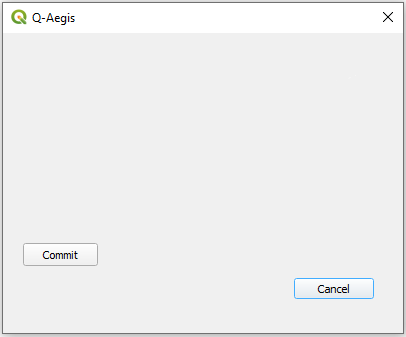
\includegraphics[width=0.8\textwidth,height=250px]{images/norepo_state.png}
	\caption{A kezelőfelület alapállapota}
	\label{fig:picture-3}
\end{figure}
Az ablak a "Cancel" gombbal zárható be, a többi gomb funkciójára, valamint a felület esetleges változásaira a használatot magyarázó részekben térünk ki.
\subsection{Új követett projekt létrehozása}
Amennyiben teljesen üres projekttel szeretnénk elkezdeni a munkát, technikai okokból a projektet létre kel hozni, elmenteni, majd újra megnyitni. Ekkor létrejön a projekthez tartozó tároló, a verziókezelés használható innentől.
Ha már meglévő projektet szeretnénk verziókezeltté tenni, akkor a projektfájl megnyitása után a kezelőfelületen található "Commit" gombra kattintva a projekt teljes állapota bekerül a rendszerbe és a további módosítások már követhetőek lesznek.

\subsection{Módosítások mentése a verziókezelőbe}
Miután módosításokat végeztünk a projekten, a "Commit" gomb újbóli megnyomásával az új állapot bekerül a revíziókezelő rendszerbe. A QGIS szerkesztési funkciói még nincsenek teljes mértékben támogatva a Q-Aegisben, a kezelt módosítások a következőek:
\begin{list}{}{}
	\item $\bullet$ Új réteg hozzáadása
	\item $\bullet$ Létező réteg eltávolítása
	\item $\bullet$ Geometria hozzáadása réteghez
	\item $\bullet$ Geometria eltávolítása rétegről
	\item $\bullet$ Geometria módosítása :
		\subitem $\bullet$ Tetszőleges geometria részének vagy egészének eltolása
		\subitem $\bullet$ Vonal típusú geometriákba új pont felvétele, pontok eltávolítása vonalakból
		\subitem $\bullet$ Poligon típusú geometriákhoz "lyukak" hozzáadása vagy eltávolítása
		\subitem $\bullet$ Multigeometriákhoz részek hozzáadása vagy eltávolítása
\end{list}

\subsection{Tetszőleges verzió betöltése}
Amennyiben már van a projekthez mentett verzió, a kezelőfelület némileg megváltozik, megjelenik rajta egy lista az elérhető verziókról (~\ref{fig:picture-4}). A listából egy tetszőleges számú verziót kiválasztva, majd a "Load Version" gombra kattintva a projektbe betöltődik a kiválasztott verzió. Amennyiben a betöltés előtt a projektben vannak olyan módosítások, amelyek még nem kerültek be a rendszerbe, a program egy felugró ablakkal figyelmezteti a felhasználót, és felajánlja neki a lehetőséget, hogy commitolja a módosításait, mielőtt betöltené az új verziót.

Ha korábbi állapot van betöltve, és módosításokat végzünk rajta, akkor ha menteni próbálunk, a rendszer hibaüzenettel jelzi, hogy előbb a legfrissebb verzióra kell állni és utána lehet módosítani.
\begin{figure}[H]
	\centering
	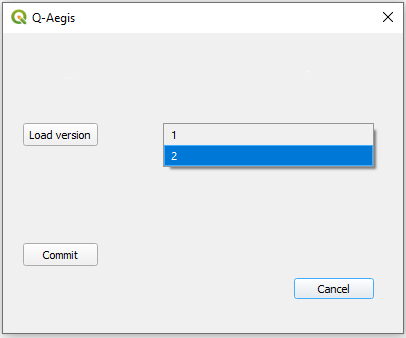
\includegraphics[width=0.8\textwidth,height=250px]{images/available_versions.png}
	\caption{A verzióválasztó lista}
	\label{fig:picture-4}
\end{figure}

\subsection{Megjegyzés a használható rétegekhez}
A QGIS több opcióval is rendelkezik arra, hogy milyen módon tároljuk a rétegeinket. A Q-Aegis csak a vektoros rétegtípusokon végzett műveleteket támogatja. Szerkesztés közben nem számít, hogy memóriában tárolt ideiglenes réteggel, vagy shapefile-ban tárolt réteggel dolgozunk, viszont verzió betöltésekor az összes réteg törlődik, és a betöltendő verziónak megfelelő rétegek jönnek létre, amik mind memóriában tároltak. Mivel alapvetően ezeket a QGIS nem tárolja, kilépéskor figyelmezteti a felhasználót, hogy ezek tartalma el fog veszni, ez viszont nem érinti azokat a projekteket, amik a Q-Aegisben vannak, hiszen az abban tárolt állapotok alapján tölti vissza az adatokat.

\subsection{Verziókezelt projekt betöltése}
A Q-Aegis jelenleg még nem ad lehetőséget arra, hogy létező tárolóból hozzunk létre egy új QGIS projektet, de az alábbi lépésekkel ez megvalósítható:
\begin{enumerate}
	\item Hozzunk létre egy új projektet, mentsük el
	\item Nyissuk meg, majd zárjuk be, így létrehozva egy új, üres tárolót
	\item Lépjünk be a telepítésnél bemásolt könyvtárban található repositories mappába (/plugins/qaegis/repositories)
	\item A másolni kívánt projekt nevével megegyező nevű konyvtár tartalmát másoljuk ki
	\item Szúrjuk be a kimásolt állományokat és alkönyvtárakat az új projekt nevével megegyező nevű mappába, felülírva tartalmát
	\item Az új projektet megnyitva rendelkezésre áll a projekt másolata
\end{enumerate}
	
\section{A modul eltávolítása}
A Q-Aegis modul kikapcsolható a QGIS beépülő modulokat kezelő felületén, ugyanúgy ahogy hozzáadásra került. A teljes eltávolításhoz töröljük ki a qaegis mappát a plugin könyvtárból.
	
